\documentclass[12pt]{article}

\usepackage[margin=1in]{geometry}
\usepackage{amsmath}
\usepackage{booktabs}
\usepackage{array}
\usepackage{graphicx}
\usepackage{listings}
\usepackage{xcolor} 

\lstset{
    language=Python,
    basicstyle=\ttfamily\small,
    keywordstyle=\color{blue}\bfseries,
    commentstyle=\color{gray}\itshape,
    stringstyle=\color{orange},
    showstringspaces=false,
    breaklines=true,
    frame=single,
    numbers=left,
    numberstyle=\tiny\color{gray},
    stepnumber=1
}

\title{DASC 605 -- Homework 1}
\author{Liam Whitenack}
\date{}

\begin{document}

\maketitle

Please complete the following exercises either on your own or within a group of up to 4 students. Each group should submit only one, typed written submission. You can submit a word file, a pdf file or a markdown file that shows the code, results and interpretations for each exercise. Make sure that if you only submit a notebook type file, you annotate the results and interpretations as applicable. I will not give full credit for submissions that only have the code or the code plus results. Interpretations and/or answers with complete sentences that are context-aware for the exercise at hand are also required to receive full credit.

\bigskip

\textbf{Total Points for this Assignment: 100}

\bigskip

Assignment should be uploaded to CANVAS page no later than 5pm on March 15.

\section*{Problem 1 [20 points]}

We want to estimate the mean number of miles driven ($\mu_y$) to work by the heads of households for homeowners in a popular subdivision within the heart of VA Beach called Cluster Ridge. Because we believe that outliers may exist in the population due to overzealous commuters, our statistic of choice will be the 20\% trimmed sample mean, tsm(.20) (which is the mean of the middle 60\% of the data in your sample: order the sample from smallest to largest and then chop off the lower 20\% of the data as well as the upper 20\% of the data, then take the sample mean of what is left).

To collect our data we will sample homes from two blocks within our subdivision, independently. Within the first block we will take a simple random sample of three of the four homes (labeled $H_1, H_2, H_3$ and $H_4$). From the second block we will independently sample two of the 6 homes (labeled $H_A, H_B, H_C, H_D, H_E, H_F$) according to the sampling design:

\begin{center}
\begin{tabular}{cc}
\toprule
Sample $S$ & $P(S)$ \\
\midrule
$\{H_A,H_C\}$ & $1/4$ \\
$\{H_B,H_D\}$ & $7/16$ \\
$\{H_A,H_E\}$ & $3/16$ \\
$\{H_C,H_F\}$ & $1/8$ \\
\bottomrule
\end{tabular}
\end{center}

The table of values for travelling distances (commuter distance) is given below along with miles per gallon for the vehicle:

\begin{center}
\begin{tabular}{ccc}
\toprule
House & Travel Distance & MPG for Car Used \\
\midrule
$H_1$ & 35 & 25 \\
$H_2$ & 50 & 20 \\
$H_3$ & 20 & 10 \\
$H_4$ & 8 & 26 \\
$H_A$ & 5 & 15 \\
$H_B$ & 15 & 20 \\
$H_C$ & 22 & 10 \\
$H_D$ & 58 & 30 \\
$H_E$ & 35 & 24 \\
$H_F$ & 50 & 27 \\
\bottomrule
\end{tabular}
\end{center}

Here is a table for the 16 possible samples one could draw with this scheme:

\begin{center}
\begin{tabular}{llllll}
\toprule
Sample $S$ & $P(S)$ & Values & $tsm(.20)$ Dist. & $tsm(.20)$ MPG & Conf.\ Interval \\
\midrule
$\{H_1,H_2,H_3,H_A,H_C\}$ & $1/16$ & $(35,50,20,5,22)$ & $25\;2/3$ & $15$ & $(19\;2/3,31\;2/3)$ \\
$\{H_1,H_2,H_3,H_B,H_D\}$ & $7/64$ & $(35,50,20,15,58)$ & $35$ & $21\;2/3$ & $(29,41)$ \\
$\{H_1,H_2,H_3,H_A,H_E\}$ & $3/64$ & $(35,50,20,5,35)$ & $30$ & $19\;2/3$ & $(24,36)$ \\
$\{H_1,H_2,H_3,H_C,H_F\}$ & $1/32$ & $(35,50,20,22,50)$ & $35\;2/3$ & $18\;1/3$ & $(29\;2/3,41\;2/3)$ \\

$\{H_1,H_2,H_4,H_A,H_C\}$ & $1/16$ & $(35,50,8,5,22)$ & $21\;2/3$ & $20$ & $(15\;2/3,27\;2/3)$ \\
$\{H_1,H_2,H_4,H_B,H_D\}$ & $7/64$ & $(35,50,8,15,58)$ & $33\;1/3$ & $23\;2/3$ & $(27\;1/3,39\;1/3)$ \\
$\{H_1,H_2,H_4,H_A,H_E\}$ & $3/64$ & $(35,50,8,5,35)$ & $26$ & $23$ & $(20,32)$ \\
$\{H_1,H_2,H_4,H_C,H_F\}$ & $1/32$ & $(35,50,8,22,50)$ & $35\;2/3$ & $23\;2/3$ & $(29\;2/3,41\;2/3)$ \\

$\{H_1,H_3,H_4,H_A,H_C\}$ & $1/16$ & $(35,20,8,5,22)$ & $16\;2/3$ & $16\;2/3$ & $(10\;2/3,22\;2/3)$ \\
$\{H_1,H_3,H_4,H_B,H_D\}$ & $7/64$ & $(35,20,8,15,58)$ & $23\;1/3$ & $23\;2/3$ & $(17\;1/3,29\;1/3)$ \\
$\{H_1,H_3,H_4,H_A,H_E\}$ & $3/64$ & $(35,20,8,5,35)$ & $21$ & $21\;1/3$ & $(15,27)$ \\
$\{H_1,H_3,H_4,H_C,H_F\}$ & $1/32$ & $(35,20,8,22,50)$ & $25\;2/3$ & $20\;1/3$ & $(19\;2/3,31\;2/3)$ \\

$\{H_2,H_3,H_4,H_A,H_C\}$ & $1/16$ & $(50,20,8,5,22)$ & $16\;2/3$ & $15$ & $(10\;2/3,22\;2/3)$ \\
$\{H_2,H_3,H_4,H_B,H_D\}$ & $7/64$ & $(50,20,8,15,58)$ & $28\;1/3$ & $22$ & $(22\;1/3,34\;1/3)$ \\
$\{H_2,H_3,H_4,H_A,H_E\}$ & $3/64$ & $(50,20,8,5,35)$ & $21$ & $19\;2/3$ & $(15,27)$ \\
$\{H_2,H_3,H_4,H_C,H_F\}$ & $1/32$ & $(50,20,8,22,50)$ & $30\;2/3$ & $18\;2/3$ & $(24\;2/3,36\;2/3)$ \\
\bottomrule
\end{tabular}
\end{center}

\begin{lstlisting}
first_block_houses = ["H1", "H2", "H3", "H4"]
first_block_samples = list(combinations(first_block_houses, 3))
first_block_probability = 1 / 4


def trimmed_mean_20(values):

    sorted_values = sorted(values)

    # remove smallest and largest
    trimmed = sorted_values[1:-1]

    return sum(trimmed) / len(trimmed)


rows = []

for first_sample in first_block_samples:

    for second_sample, second_probability in second_block_probabilities.items():

        sample = list(first_sample) + list(second_sample)

        probability = first_block_probability * second_probability

        distances = [travel_distance[h] for h in sample]
        mpgs = [mpg_for_car_used[h] for h in sample]

        tsm_distance = trimmed_mean_20(distances)
        tsm_mpg = trimmed_mean_20(mpgs)

        confidence_interval = (tsm_distance - 6, tsm_distance + 6)

        rows.append(
            {
                "Sample": sample,
                "P(S)": probability,
                "Values": distances,
                "tsm(.20) Distance": tsm_distance,
                "tsm(.20) MPG": tsm_mpg,
                "Conf Interval": confidence_interval,
            }
        )
\end{lstlisting}

\begin{enumerate}
\item[(a)] Is tsm(.20) unbiased for the population average commute distance? If not, what is the bias?

\begin{lstlisting}
expected_tsm_distance = (table["tsm(.20) Distance"] * table["P(S)"]).sum()
true_average = mean(list(travel_distance.values()))

bias_distance_mean = expected_tsm_distance - true_average
\end{lstlisting}

\[
\text{Bias}(tsm_{.20}) = E(tsm_{.20}) - \mu
\]

\[
= 26.645833333333332 - 29.8
\]

\[
= -3.154166666666668
\]

\textit{\textcolor{blue}{Thus, the estimator tsm(.20) is biased and underestimates the true population mean commute distance by approximately $3.154$ miles on average.}}
\item[(b)] Is tsm(.20) unbiased for the 20\% trimmed population commute distance? If not, what is the bias?

\begin{lstlisting}
true_tsm_20_average = mean(sorted(travel_distance.values())[2:8])

bias_distance_trimmed = expected_tsm_distance - true_tsm_20_average
\end{lstlisting}

\[
\text{Bias}(tsm_{.20}) = E(tsm_{.20}) - \mu
\]

\[
= 26.645833333333332 - 29.5
\]

\[
= -2.854166666666668
\]

\textit{\textcolor{blue}{Thus, the estimator tsm(.20) is biased and underestimates the true population mean commute distance by approximately $2.854$ miles on average.}}

\item[(c)] What is the true sampling variance for tsm(.20) for estimating commuter distance under the proposed sampling design?

\begin{lstlisting}
variance_distance = (
    table["P(S)"]
    * (table["tsm(.20) Distance"] - expected_tsm_distance) ** 2
).sum()
\end{lstlisting}

\[
\text{Var}(tsm_{.20}) = 36.650173611111114
\]

\item[(d)] What is the confidence level for the confidence interval $tsm_{.20} \pm 6$ for estimating the true mean commuting distance?

\begin{lstlisting}
coverage = table.apply(
    lambda row: row["P(S)"]
    if (true_average >= row["tsm(.20) Distance"] - 6)
    and (true_average <= row["tsm(.20) Distance"] + 6)
    else 0,
    axis=1,
).sum()
\end{lstlisting}

\[
\text{Confidence Level} = \frac{21}{32} \approx 0.65625
\]

\textit{\textcolor{blue}{Thus, the confidence interval $tsm_{.20} \pm 6$ captures the true mean commuting distance with probability $\frac{21}{32}$.}}

\item[(e)] Repeat (a) through (d) for average MPG. For part (d) what is the confidence level for the confidence interval $tsm_{.20} \pm 4$ for estimating the true mean MPG?

\begin{lstlisting}
true_mpg_mean = mean(list(mpg_for_car_used.values()))
true_mpg_trimmed = mean(sorted(mpg_for_car_used.values())[2:8])

expected_tsm_mpg = (table["tsm(.20) MPG"] * table["P(S)"]).sum()

bias_mpg_mean = expected_tsm_mpg - true_mpg_mean
bias_mpg_trimmed = expected_tsm_mpg - true_mpg_trimmed
\end{lstlisting}

\[
E(tsm_{.20}^{MPG}) = 20.765625
\]

\[
\text{Population Mean MPG} = 20.7
\]

\[
\text{Bias (Population Mean)} = 0.065625
\]

\[
\text{20\% Trimmed Population Mean MPG} = 20.5
\]

\[
\text{Bias (Trimmed Mean)} = 0.265625
\]

\begin{lstlisting}
variance_mpg = (
    table["P(S)"]
    * (table["tsm(.20) MPG"] - expected_tsm_mpg) ** 2
).sum()
\end{lstlisting}

\[
\text{Var}(tsm_{.20}^{MPG}) = 7.458740234375
\]

\begin{lstlisting}
coverage_mpg = table.apply(
    lambda row: row["P(S)"]
    if (true_mpg_mean >= row["tsm(.20) MPG"] - 4)
    and (true_mpg_mean <= row["tsm(.20) MPG"] + 4)
    else 0,
    axis=1,
).sum()
\end{lstlisting}

\[
\text{Confidence Level} = \frac{59}{64} \approx 0.921875
\]

\textit{\textcolor{blue}{Thus, the interval $tsm_{.20} \pm 4$ captures the true mean MPG with probability $\frac{59}{64}$.}}

\end{enumerate}

\section*{Problem 2 [20 points]}

For independent $Y_1 \sim Binomial(n_1,\pi_1)$ and $Y_2 \sim Binomial(n_2,\pi_2)$, the quantity $\hat{\pi}_1/\hat{\pi}_2$ is called the \textit{relative risk} or \textit{risk ratio}. This measure is often used in medical research to compare the probability of a certain outcome for two treatments.

A randomized study with $n_1=n_2=50$ compares the probabilities of success $\pi_1$ for a new drug and $\pi_2$ for placebo. Suppose $\pi_1=0.20$ and $\pi_2=0.10$.

\vspace{1cm}
\textit{Python code below was used to simulate sample proportions and generate histograms.}
\begin{lstlisting}
import matplotlib.pyplot as plt
import numpy as np
from numpy import errstate, isfinite, log, ndarray
from numpy.random import binomial


def get_risk_ratio(n1: int, n2: int) -> tuple[ndarray, ndarray]:
    y1 = binomial(n1, 0.20, 1_000_000)
    y2 = binomial(n2, 0.10, 1_000_000)

    pi1_hat = y1 / 50
    pi2_hat = y2 / 50

    with errstate(divide="ignore", invalid="ignore"):
        risk_ratio = pi1_hat / pi2_hat
        log_risk_ratio = log(risk_ratio)

    # keep only valid values
    risk_ratio = risk_ratio[isfinite(risk_ratio)]
    log_risk_ratio = log_risk_ratio[isfinite(log_risk_ratio)]

    return risk_ratio, log_risk_ratio


def histogram(n1: int, n2: int, fname: str) -> None:
    risk_ratio, log_risk_ratio = get_risk_ratio(n1, n2)

    combined = np.concatenate([risk_ratio, log_risk_ratio])
    bins = np.linspace(combined.min(), combined.max(), 101)

    plt.hist(risk_ratio, bins=bins, alpha=0.5, label="Risk Ratio")
    plt.hist(log_risk_ratio, bins=bins, alpha=0.5, label="Log Risk Ratio")

    plt.title(fname)

    plt.legend()

    plt.savefig(f"plots/{fname.replace(' ', '_')}.png")
    plt.close()
\end{lstlisting}

\begin{enumerate}
\item[(a)] Simulate 1,000,000 sample proportions from each treatment with $n_1=n_2=50$. Construct histograms for $\hat{\pi}_1/\hat{\pi}_2$ and $\log(\hat{\pi}_1/\hat{\pi}_2)$. Which seems to have sampling distribution closer to normality?  

\textit{\textcolor{blue}{The risk ratio is strongly right-skewed; the log risk ratio is approximately symmetric and closer to normal.  }}

\begin{center}
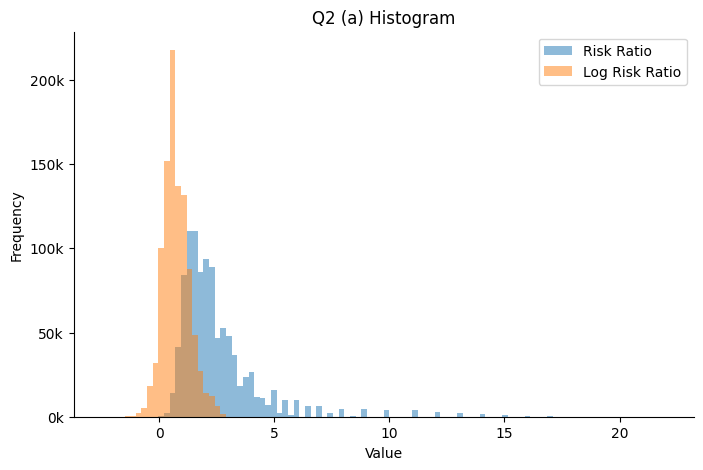
\includegraphics[width=0.7\textwidth]{plots/Q2_a_Histogram.png}
\end{center}

\item[(b)] Simulate 1,000,000 sample proportions from each treatment with $n_1=n_2=1000$. Construct histograms for $\hat{\pi}_1/\hat{\pi}_2$ and $\log(\hat{\pi}_1/\hat{\pi}_2)$. Which seems to have sampling distribution closer to normality? Is this answer consistent with part (a)?  

\textit{\textcolor{blue}{Larger samples make both distributions more normal; the log risk ratio remains closer to normal. This is consistent with part (a).  }}

\begin{center}
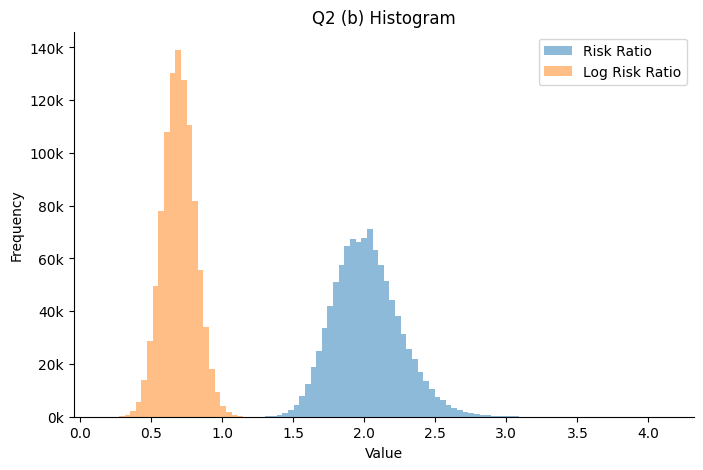
\includegraphics[width=0.7\textwidth]{plots/Q2_b_Histogram.png}
\end{center}

\item[(c)] Repeat step (a) but assume $n_1=30$ and $n_2=70$. What do the empirical sampling distributions suggest about normality? Is this as clear as part (a)?  

\textit{\textcolor{blue}{Unequal samples increase skew; the log risk ratio is still more symmetric but less clearly normal.  }}

\begin{center}
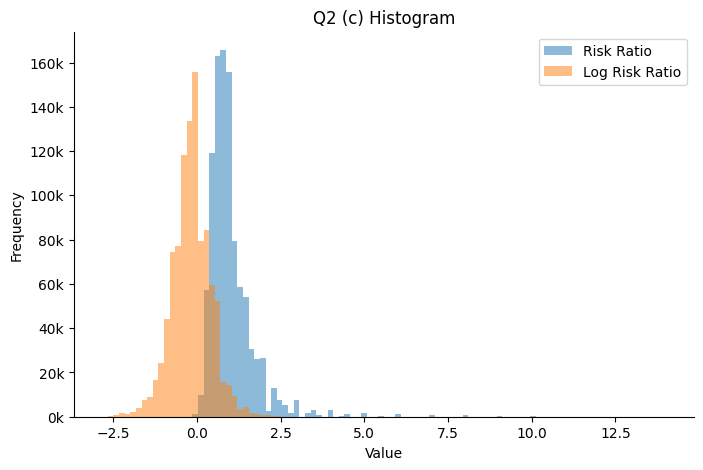
\includegraphics[width=0.7\textwidth]{plots/Q2_c_Histogram.png}
\end{center}

\item[(d)] Repeat step (c) but now with sample sizes $n_1=70$ and $n_2=30$.  

\textit{\textcolor{blue}{Small denominator sample exaggerates skew in the risk ratio; the log risk ratio remains closer to normal, though slight skewness remains.  }}

\begin{center}
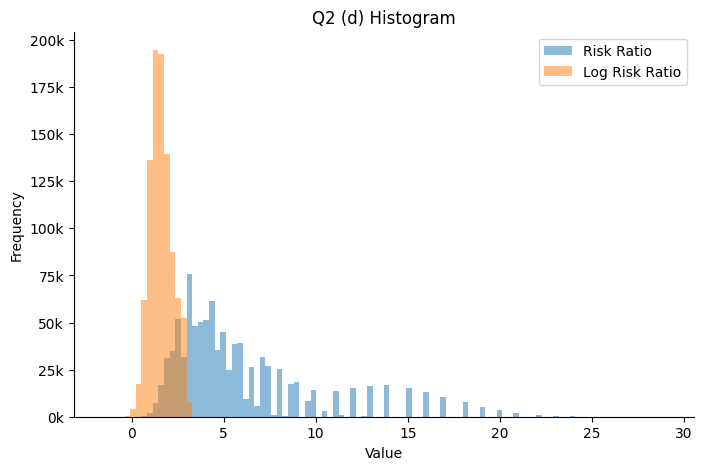
\includegraphics[width=0.7\textwidth]{plots/Q2_d_Histogram.png}
\end{center}
\end{enumerate}

\section*{Problem 3 [20 points]}

For a point estimate of the mean of a population that is assumed to have a normal distribution, a data scientist decides to use the average of the sample lower and upper quartiles for the $n=100$ observations, since unlike the sample mean $\bar{Y}$, the quartiles are not affected by outliers.

\begin{enumerate}

\item[(a)] Evaluate the precision of this estimator compared to $\bar{Y}$ by randomly generating 100,000 samples of size 100 each from a $N(0,1)$ distribution and comparing the standard deviation of the 100,000 estimates with the theoretical standard error of $\bar{Y}$.

\begin{lstlisting}
def simulate_precision(n: int) -> None:
    samples = rng.normal(loc=0, scale=1, size=(100_000, n))
    quartile_estimates = [quartile_mean_estimator(sample) for sample in samples]
    mean_estimates = samples.mean(axis=1)
    std_quartile = np.std(quartile_estimates, ddof=1)
    std_mean = np.std(mean_estimates, ddof=1)
    se_mean = 1 / np.sqrt(n)

    print(f"Sample size: {n}")
    print(f"Quartile-based estimator std dev: {std_quartile}")
    print(f"Sample mean std dev: {std_mean}")
    print(f"Theoretical standard error of mean: {se_mean}")
    print("\n")
\end{lstlisting}

\textit{\textcolor{blue}{Simulation results:}}

\begin{verbatim}
Sample size n = 100
Quartile-based estimator std dev: 0.11021916844201737
Sample mean std dev: 0.0997464865829455
Theoretical standard error of mean: 0.1
\end{verbatim}

\textit{\textcolor{blue}{The quartile-based estimator has a standard deviation of $0.1102$, which is larger than the theoretical standard error of $\bar{Y}$ ($0.1$). Thus, for a normal population the quartile estimator is less precise than the sample mean.}}

\item[(b)] Evaluate the precision of this estimator compared to $\bar{Y}$ by randomly generating 100,000 samples of size 500 each from a $N(0,1)$ distribution and comparing the standard deviation of the 100,000 estimates with the theoretical standard error of $\bar{Y}$.

Simulation results:

\begin{verbatim}
Sample size n = 500
Quartile-based estimator std dev: 0.04953018659979792
Sample mean std dev: 0.044660325627139806
Theoretical standard error of mean: 0.044721359549995794
\end{verbatim}

\textit{\textcolor{blue}{Again, the quartile-based estimator has a larger standard deviation (0.0495) than the sample mean, 0.0447. The difference is smaller with larger $n$, but the sample mean remains the more precise estimator for a normal distribution.}}

\end{enumerate}
\section*{Problem 4a [15 points]}


\textit{\textcolor{blue}{We construct 95\% confidence intervals for the population proportions using the Wald (normal approximation) method implemented in \texttt{statsmodels}:}}

\begin{lstlisting}
male_lower, male_upper = proportion_confint(
    count=703,
    nobs=945,
    alpha=0.05,
    method="normal",
)

female_lower, female_upper = proportion_confint(
    count=1017,
    nobs=1178,
    alpha=0.05,
    method="normal",
)
\end{lstlisting}

\textit{\textcolor{blue}{This yields the following intervals:}}

\[
\text{Male CI: } (0.7161, 0.7717)
\]

\[
\text{Female CI: } (0.8437, 0.8829)
\]

\textit{\textcolor{blue}{The 95\% confidence interval for males indicates that we are 95\% confident that between $71.6\%$ and $77.2\%$ of males in the population believe in life after death. The 95\% confidence interval for females indicates that we are 95\% confident that between $84.4\%$ and $88.3\%$ of females believe in life after death.}}

\textit{\textcolor{blue}{Figure~\ref{fig:normal_ci} shows the confidence intervals for both groups.}}

\begin{figure}[h]
\centering
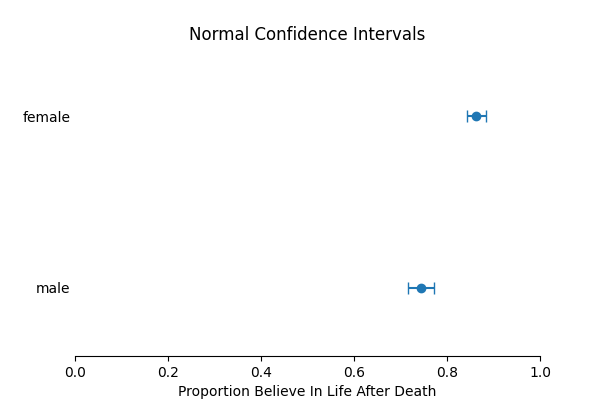
\includegraphics[width=0.7\textwidth]{plots/Normal_Confidence_Intervals.png}
\caption{95\% Wald confidence intervals for the proportions of males and females who believe in life after death.}
\label{fig:normal_ci}
\end{figure}

\textit{The intervals do not overlap, suggesting that the population proportion of females who believe in life after death is higher than the proportion of males.}
\section*{Problem 4b [25 points]}
Using any dataset from the repository:

\texttt{https://stat4ds.rwth-aachen.de/data/}

complete the following ``mini report'' that will include:


\begin{enumerate}

\item[(i)] Description of the problem you are trying to solve -- estimation goals for the project and background on why this is important. Assume 90\% confidence levels for all estimates.

\textit{\textcolor{blue}{The goal of this project is to determine which demographic categories are associated with higher happiness levels. In particular, we examine whether happiness varies across marital status and sex categories. For example, \texttt{mean\_happiness = df['happiness'].mean()} gives a quick summary of the outcome.}}

\textit{\textcolor{blue}{Understanding which groups report higher happiness can provide insight into how social factors influence well-being. You might start with \texttt{df.groupby('marital')['happiness'].mean()} to explore trends.}}

\textit{\textcolor{blue}{Unless otherwise specified, all interval estimates use 90\% confidence levels, e.g., \texttt{ci\_lower, ci\_upper = mean\_confidence\_interval(df['happiness'], confidence=0.90)}.}}

\item[(ii)] Description of the data you will use to solve the problem and discussion of key variables.

\textit{\textcolor{blue}{The dataset contains the following variables:}}

\begin{itemize}
\item \textit{\textcolor{blue}{\texttt{id}: unique respondent identifier, e.g., \texttt{ids = df['id'].unique()}}}
\item \textit{\textcolor{blue}{\texttt{happiness}: categorical happiness score (1-3), e.g., \texttt{df['happiness'].value\_counts()}}}
\item \textit{\textcolor{blue}{\texttt{marital}: marital status category (1-3), e.g., \texttt{df.groupby('marital')['happiness'].mean()}}}
\item \textit{\textcolor{blue}{\texttt{sex}: respondent sex ("male" or "female"), e.g., \texttt{df['sex'].unique()}}}
\end{itemize}

\textit{\textcolor{blue}{Happiness and marital status are ordinal categorical variables where larger values represent greater happiness. \texttt{df.describe()} helps summarize this.}}

\textit{\textcolor{blue}{Sample size: \texttt{len(df)} = 2142}}

\item[(iii)] Depiction of the sample data distribution for each variable you are considering. If the outcome is categorical, give a bar chart of the sample distribution.

\textit{\textcolor{blue}{Bar charts show the distribution of each categorical variable. You can generate them with \texttt{df['happiness'].value\_counts().plot(kind='barh')} or the \texttt{barchart()} helper function.}}

\begin{figure}[h!]
    \centering
    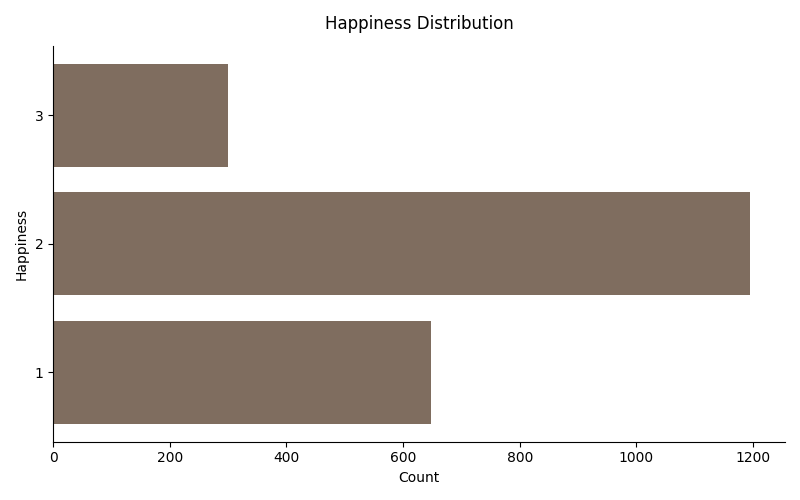
\includegraphics[width=0.7\textwidth]{plots/happiness_distribution.png}
    \caption{Distribution of happiness scores, e.g., \texttt{barchart(x=counts.index, y=counts.values, y\_label='Happiness')}}.
\end{figure}

\begin{figure}[h!]
    \centering
    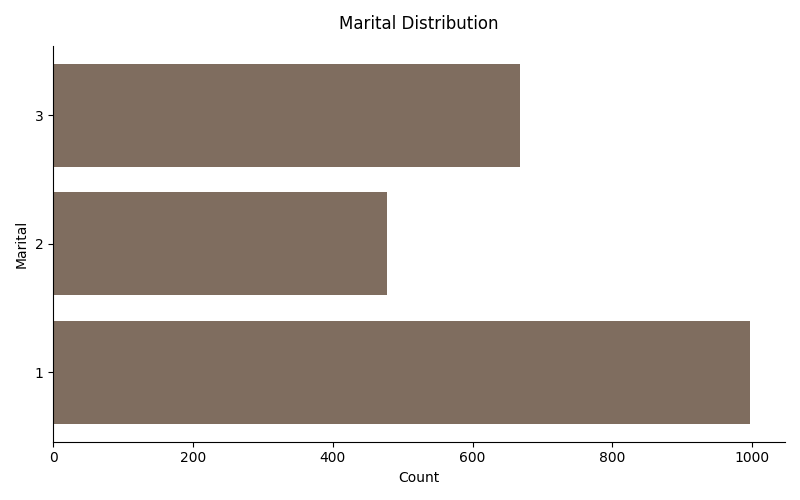
\includegraphics[width=0.7\textwidth]{plots/marital_distribution.png}
    \caption{Distribution of marital status, e.g., \texttt{barchart(x=df['marital'].unique(), y=df['marital'].value\_counts())}}.
\end{figure}

\begin{figure}[h!]
    \centering
    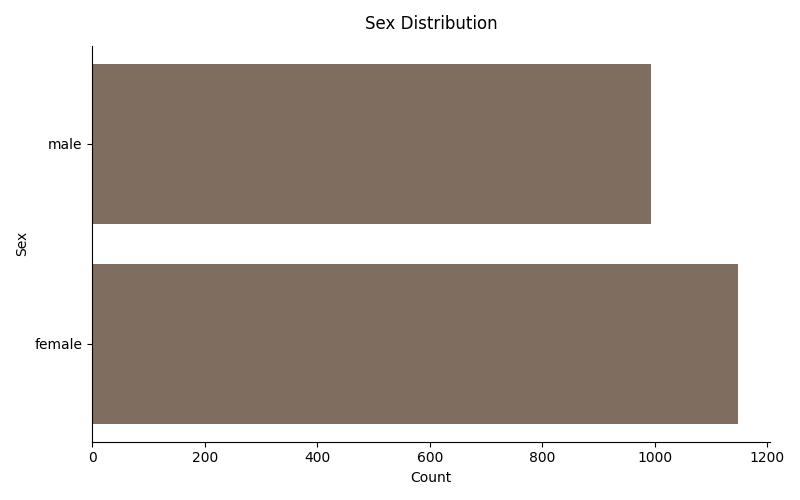
\includegraphics[width=0.7\textwidth]{plots/sex_distribution.png}
    \caption{Distribution of sex, e.g., \texttt{df['sex'].value\_counts().plot(kind='barh')}}.
\end{figure}

\item[(iv)] Estimation involving at least one mean and one proportion (with point and interval estimates) and their interpretation.

\textit{\textcolor{blue}{The estimated mean happiness score is 1.837 (\texttt{mean\_happiness = df['happiness'].mean()}).}}

\textit{\textcolor{blue}{The 90\% confidence interval for the population mean happiness is (1.814, 1.860) (\texttt{ci\_lower, ci\_upper = mean\_confidence\_interval(df['happiness'])}).}}

\textit{\textcolor{blue}{We are 90\% confident that the true population average happiness lies within this interval.}}

\textit{\textcolor{blue}{The estimated proportion of individuals reporting the highest happiness (level 3) is 0.140 (\texttt{p\_hat = (df['happiness'] == 3).mean()}).}}

\textit{\textcolor{blue}{The 90\% confidence interval for this proportion is (0.127, 0.152) (\texttt{proportion\_confidence\_interval(count=happy\_count, n=len(df))}).}}

\item[(v)] Estimation involving two groups compared on their averages or proportions.

\textit{\textcolor{blue}{Mean and median happiness by sex: \texttt{group\_stats = df.groupby('sex')['happiness'].agg(['mean','median','count'])}.}}

\begin{table}[h!]
\centering
\begin{tabular}{lccc}
\toprule
sex & mean & median & count \\
\midrule
female & 1.825784 & 2.0 & 1148 \\
male   & 1.850101 & 2.0 & 994 \\
\bottomrule
\end{tabular}
\caption{Happiness by sex.}
\end{table}

\textit{\textcolor{blue}{The difference between the highest and lowest mean happiness across sex categories is 0.024 (\texttt{mean\_diff = group\_stats['mean'].max() - group\_stats['mean'].min()}).}}

\textit{\textcolor{blue}{To examine whether these differences are meaningful, we plot the mean happiness scores by marital status and sex along with 90\% confidence intervals, e.g., \texttt{plot\_happiness\_by\_marital\_sex(df)}.}}

\begin{figure}[h!]
    \centering
    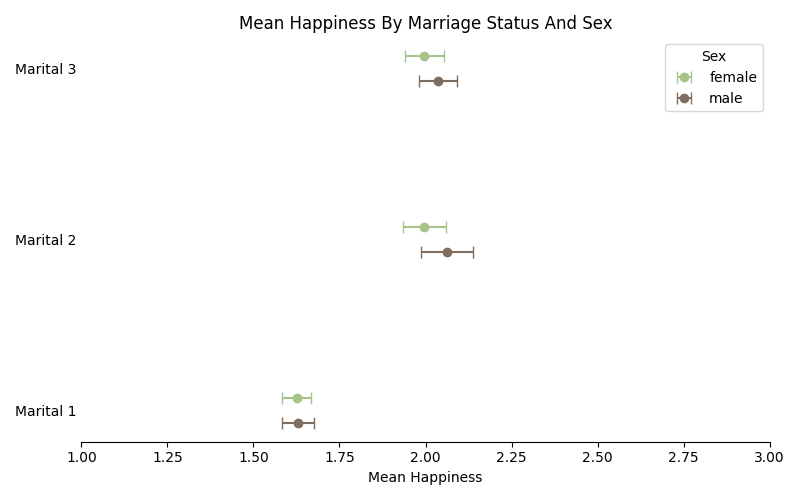
\includegraphics[width=0.7\textwidth]{plots/mean_happiness_by_marriage_status_and_sex.png}
    \caption{Mean happiness by marital status and sex with 90\% confidence intervals.}
\end{figure}

\item[(vi)] A 95\% confidence interval for the correlation between two continuous variables along with a corresponding scatterplot. Use bootstrapping with 1000 bootstrap samples.

\textit{\textcolor{blue}{We estimate the correlation between marital status and happiness. \texttt{corr = np.corrcoef(df['happiness'], df['marital'])[0,1]}.}}

\textit{\textcolor{blue}{A 95\% bootstrap confidence interval is constructed using 1000 bootstrap samples, e.g., \texttt{corr\_boot = bootstrap\_correlation(df['happiness'].to\_numpy(), df['marital'].to\_numpy())}.}}

\textit{\textcolor{blue}{The estimated correlation is 0.274.}}

\textit{\textcolor{blue}{The 95\% bootstrap confidence interval is (0.236, 0.315).}}

\item[(vii)] For one continuous outcome, compute a 95\% confidence interval of the Karl Pearson Skewness coefficient:

\[
3(\text{mean}-\text{median})/\text{standard deviation}
\]

based on 1000 bootstrap samples. Provide the interval and a visualization of the bootstrap distribution.

\textit{\textcolor{blue}{The estimated skewness is -0.758 (\texttt{pearson\_skew(df['happiness'])}).}}

\textit{\textcolor{blue}{The 95\% bootstrap confidence interval is (-0.883, -0.615) (\texttt{skew\_boot = [pearson\_skew(rng.choice(df['happiness'], size=len(df), replace=True)) for \_ in range(1000)]}).}}

\begin{figure}[h!]
    \centering
    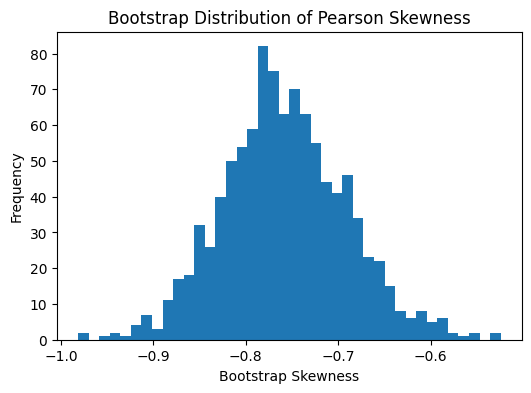
\includegraphics[width=0.6\textwidth]{plots/skewness_bootstrap.png}
    \caption{Bootstrap distribution of Pearson skewness estimates.}
\end{figure}

\item[(viii)] A closing section highlighting what you learned from the data relative to your goals.

\textit{\textcolor{blue}{Provided that my assumptions about the data are correct, I did achieve my goals in analyzing the data. Small code snippets like \texttt{df.groupby(['marital','sex'])['happiness'].mean()} help reveal which groups report higher happiness.}}

\textit{\textcolor{blue}{It is obvious that the marital status of "1" is detrimental to the happiness score, while the other feature, "sex", does not seem to make a substantial difference.}}

\end{enumerate}




\end{document}